\definecolor{codegray}{rgb}{0.5,0.5,0.5}
\lstdefinestyle{mystyle}{
    commentstyle=\color{codegray},
    numberstyle=\tiny\color{codegray},
    basicstyle=\ttfamily\footnotesize,
    breakatwhitespace=false,         
    breaklines=true,                 
    captionpos=b,                    
    keepspaces=true,                 
    numbers=left,                    
    numbersep=5pt,                  
    showspaces=false,                
    showstringspaces=false,
    showtabs=false,                  
    tabsize=2
}
\lstset{style=mystyle}

\lstdefinelanguage{AMPL}{keywords={set,param,var,arc,integer,minimize,maximize,subject,to,node,sum,in,Current,complements,integer,solve_result_num,IN,contains,less,suffix,INOUT,default,logical,sum,Infinity,dimen,max,symbolic
,Initial,div,min,table,LOCAL,else,option,then,OUT,environ,setof ,union,all,exists,shell_exitcodeuntil,binary,forall,solve_exitcodewhile ,by,if,solve_messagewithin,check,in,solve_result
},sensitive=true,comment=[l]{\#}}

\lstset{frame=tb,
  language=AMPL,
  aboveskip=3mm,
  belowskip=3mm,
  showstringspaces=false,
  columns=flexible,
  basicstyle={\ttfamily},
  numbers=none,
  numberstyle=\tiny\color{gray},
  keywordstyle=\bfseries,
  commentstyle=\textit,
  stringstyle=\color{mauve},
  breaklines=true,
  breakatwhitespace=true,
  tabsize=3
}
\titleformat{\chapter}[display]
    {\normalfont\Large\bfseries}{\filleft\chaptertitlename\ \thechapter}{20pt}{\Huge}
\chapter{Análisis del problema planteado}
    \justify    
        Como se menciona en un inicio, el \textbf{TSP} o ``\textit{Travelling Salesman Problem}" lleva varias décadas siendo investigado es por esto que es fundamental hacer una mirada retrospectiva. 
        
        \section{Contexto histórico}
            Sus inicios se remontan aparentemente más allá de los 1900, por otro lado, dentro de la programación fue incorporado luego de 1950 como un problema de ``\textit{Programación Lineal en Enteros}'' donde se logra resolver el problema para 42 ciudades, óptimamente \parencite{WikipediaTSP}.
            \newline
            \newline
            Años más tarde, en 1972 Richard Karp demuestra que un \textit{ciclo hamiltoniano} es de complejidad \textbf{NP-Completo} lo cual implicaría que el \textbf{TSP} es de complejidad \textbf{NP-HARD}.
            
        \section{Descripción del problema}
            De esta manera, desde que se tiene conocimiento del \textbf{TSP} se han ido implementando distintas heurísticas y se han realizado además un sinfín de metodologías y cálculos matemáticos para encontrar nuevas soluciones para cantidades de nodos cada vez mayores, como se puede apreciar en la \textit{Figura 2.1}.
            \begin{figure}[ht]
                \centering
                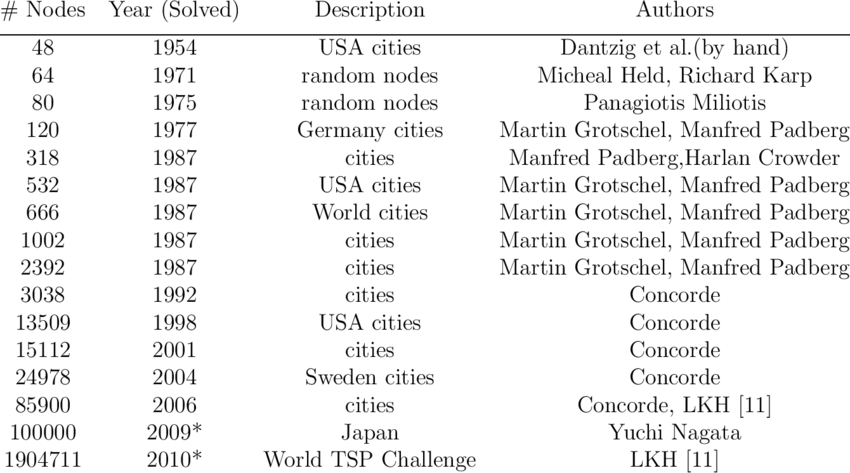
\includegraphics{imgs/TSP-Records-Variation-By-Years-3.png}
                \caption{TSP Records Variation By Years\parencite{np}}
                \label{Ilustracion 1}
            \end{figure}
            \newline
            Como se menciona previamente, el ``problema del vendedor viajero'' o \textbf{TSP} es un problema matemático el cual hace referencia a la problemática de encontrar la ruta más corta y, al mismo tiempo la más eficiente para llegar a un destino.  
            \newline
            \newline
            También se menciona que gracias a la investigación de Richard Karp en 1972 se determina que es de complejidad \textbf{NP-Hard}, eso quiere decir que aún no se encuentra un algoritmo de orden polinomial, es decir, un algoritmo que resuelva el problema en un tiempo prudente.  
            \newline
            \newline
            Cuando se habla de un algoritmo que resuelva un problema en un tiempo prudente o se habla de un algoritmo eficiente, se refiere a que el problema debe ser a lo más, de orden o complejidad exponencial (\(O^n\)). 
            \newline
            \newline
            En cuanto al \textbf{TSP}, existen dos maneras de estudiarlo, por un lado, está el \textit{TSP simétrico} el cual dice que la distancia entre un par de ciudades es la misma en cada dirección, este podría ser representado como un grafo no dirigido. Por el otro, está el \textit{TSP asimétrico} el cual plantea que pueden no existir caminos en ambas direcciones o que las distancias pueden ser diferentes, en este caso se podría representar por un grafo dirigido. 
        
        \section{Aplicación en grafos}
            Otra manera de representar TSP es mediante grafos, como se menciona previamente, pueden ser gráficos dirigidos y no dirigidos, cada uno con sus respectivas ventajas y desventajas.
                \newline
                \begin{figure}[ht]
                    \centering
                    \begin{minipage}{0.45\textwidth}
                        \centering
                        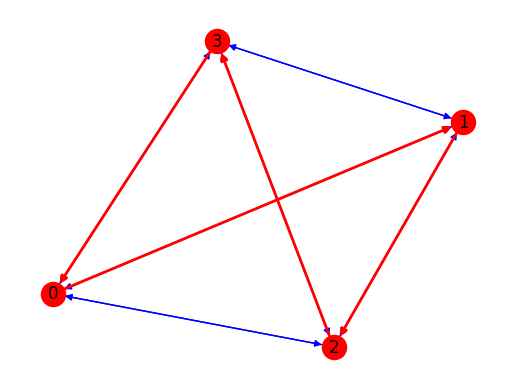
\includegraphics[scale=0.4]{imgs/Grafo_Dirigido.png}
                        \caption{Ejemplo de grafo dirigido}
                        \label{Ilustracion 5}
                    \end{minipage}\hfill
                    \begin{minipage}{0.45\textwidth}
                        \centering
                        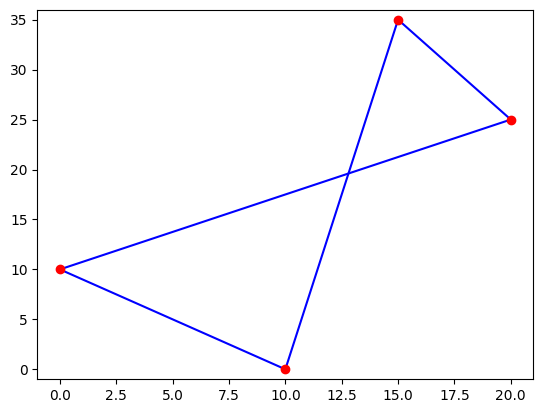
\includegraphics[scale=0.4]{imgs/Grafo_No_Dirigido.png}
                        \caption{Ejemplo de grafo no dirigido}
                        \label{Ilustracion 4}
                    \end{minipage}
                \end{figure}
                \newline
                
            \subsection{Grafos no dirigidos}
                Un grafo no dirigido es superior en términos de eficiencia y velocidad de cálculo, pues no debe diferenciar entre salida y entrada de un grafo. Además, como se menciona previamente posee simetría, es decir, se considera bidireccional por lo que no hay que almacenar dos aristas separadas.
                \newline
                \newline
                En la \textit{Figura 2.2} el grafo representa \textbf{TSP} mediante sus nodos, cada nodo representa una ciudad y cada arista representan las distancias entre ciudades. Para resolverlo se debe minimizar la distancia total del recorrido, teniendo en cuenta que se debe visitar cada nodo una sola vez.
                
            \subsection{Grafos dirigidos}
                Por el contrario, un grafo dirigido permite representar relaciones asimétricas entre nodos, esto en caso de requerir una dirección o flujo de información. Si bien pueden ser útiles para algoritmos de búsqueda en profundidad o en anchura, esto llega a consumir mucho mas almacenamiento o memoria.
                \newline
                \newline
                En la \textit{Figura 2.3} esta representado un grafo dirigido, de manera similar al grafo anterior se debe encontrar un \textit{ciclo hamiltoniano} y minimizar la longitud total del recorrido. La diferencia radica en la solución o metodología implementada, así como en el costo computacional implicado, siendo en este segundo grafo frecuentemente mayor.   
                \newline
                \newline
                En general, la implementación de grafos permite visualizar de manera mucho mas practica una solución, de esta manera se podrían estudiar los datos y establecer distintas conclusiones. Por otro lado, lo ideal al momento de trabajar con grafos es implementar heurísticas o algoritmos que reduzcan la complejidad.
                
        \section{Aplicación practica}
            Para comprender la magnitud del crecimiento del problema se puede visualizar el caso práctico presentado en \parencite{WikipediaTSP} en este caso se define en primera instancia:
                \begin{equation}
                    \frac{(n-1)!}{2}                                  
                \end{equation}
            De acuerdo al ejemplo se toman 5 ciudades y se evalúan las rutas posibles para recorrer cada ciudad una sola vez, dando como resultado 12 rutas posibles.
                \begin{equation}
                    \frac{(5-1)!}{2} = 12 \quad
                    \frac{(6-1)!}{2} = 60 \quad
                    \frac{(7-1)!}{2} = 360 \quad
                    \frac{(8-1)!}{2} = 2520 \quad                    
                \end{equation}
            De la misma manera para \(n = 6 , n=7, n= 8\) , como se muestra en la \textit{Ecuación 2.2} , donde n es  la cantidad de ciudades y el resultado es la cantidad de rutas posibles. Como se puede apreciar, si bien estos resultados pueden ser calculados directamente hasta cierto punto, el incremento de ciudades aumenta por su lado la cantidad de rutas de manera factorial. Esto se comprueba si \(n\) recibe valores mas altos que 10, como dando resultados como los de la \textit{Ecuación 2.3}, donde al aumentar \(n\) en 2 el resultado aumenta en dos cifras. 
                \begin{equation}
                    \frac{(10-1)!}{2} = 181.440 \quad
                    \frac{(12-1)!}{2} = 19.958.400 \quad
                    \frac{(14-1)!}{2} = 3.113.510.400 \quad                    
                \end{equation}
            El problema al aumentar el resultado de manera factorial se demuestra que es un problema \textbf{NP-Completo}. Mediante el mismo procedimiento se completa la Tabla 1.1 con resultados en mas instancias.
            
        \section{Paradigmas en TSP}
            Para analizar el rendimiento de una posible solución al TSP, ¿Realmente importante tener en cuenta el paradigma de programación con el que se esta trabajando? Según la pagina web \parencite{KeepCoding} “Los paradigmas de programación hacen referencia a las diferentes formas en las que se puede desarrollar un software y, al mismo tiempo, los diversos enfoques sistemáticos que pueden ser aplicados en todos los niveles del diseño de programas...” 
            \newline
            \newline
            En resumen, un paradigma de programación afecta principalmente a la complejidad del código, o mas bien, a la visualización o lectura de este. Un paradigma de programación puede facilitar o complejizar un algoritmo, en la actualidad se cuenta con 5 paradigmas, Imperativo, Orientado a objetos, Funcional, Lógico y basado en eventos. Todos con sus beneficios y desventajas, tanto para resolver TSP, como para programación en general.

                \subsection{Dialogo con ChatGPT}      

                Hoy por hoy, herramientas como ChatGPT proporcionan respuestas desde preguntas cotidianas hasta requerimientos de niveles académicos superiores, mediante deep learning y artificial intelligence proponen soluciones a través de especies de “dialogos” entre usuario bot. En definitiva, una herramienta fundamental y precisa en la actualidad, mas no infalible.
                \newline
                \newline
                Por esta razón, tanto en este caso como más adelante, se realizarán diálogos con dicha herramienta para barajar distintas propuestas para una misma consulta.
                \newline
                \newline
                Según \parencite{GPTPARADIGMAS}: “No hay un paradigma de programación específico que sea considerado el “mejor" para resolver o trabajar con el problema del TSP (Traveling Salesman Problem). La elección del paradigma depende más de los requisitos del proyecto, las preferencias personales y las características del problema en sí...”
                \newpage
                \textit{Si no tomas en cuenta las capacidades personales con respecto a los paradigmas, cual crees que es, objetivamente, ¿la mejor opción?}
                \newline
                \newline
                “Es importante tener en cuenta que la elección del “mejor" paradigma para abordar el problema del TSP no puede ser determinada de forma objetiva, ya que depende de varios factores y contextos específicos. Cada paradigma tiene sus propias fortalezas y debilidades, y la elección del mejor paradigma puede variar según el problema en particular, los recursos disponibles y los requisitos del proyecto…”
                \newline
                \newline
                “…El paradigma funcional podría ser útil para implementar algoritmos de optimización y heurísticas. La programación funcional, con su enfoque en funciones puras y datos inmutables, puede proporcionar un razonamiento declarativo y una abstracción de alto nivel para expresar operaciones de búsqueda y evaluación de soluciones…”
                \newline
                \newline
                En esta ocasión, ChatGPT presenta un punto similar al esperado, puesto que en un inicio propone que realmente ningún paradigma es superior o mas conveniente que otro en cualquier punto que NO sea de apreciación personal. Además, señala que el paradigma funcional puede llegar a ser útil para implementar algoritmos de optimización y heurísticas, esto es relevante puesto que mas adelante se implementan algoritmos que utilizan dicho paradigma.
